\specialchapter{\texorpdfstring{PLATE IX. SYSTEM OF TYPE \(\mathbf{G}_2\)}{PLATE IX. SYSTEM OF TYPE G\_2}}

\begin{enumerate}
\def\labelenumi{(\Roman{enumi})}
\tightlist
\item
  V is the hyperplane in \(E = R^{3}\) with equation \(\xi_{1} + \xi_{2} + \xi_{3} = 0\) . Roots:
\end{enumerate}

\[
\begin{array}{c} \pm (\varepsilon_ {1} - \varepsilon_ {2}), \quad \pm (\varepsilon_ {1} - \varepsilon_ {3}), \quad \pm (\varepsilon_ {2} - \varepsilon_ {3}), \quad \pm (2 \varepsilon_ {1} - \varepsilon_ {2} - \varepsilon_ {3}), \\ \pm (2 \varepsilon_ {2} - \varepsilon_ {1} - \varepsilon_ {3}), \quad \pm (2 \varepsilon_ {3} - \varepsilon_ {1} - \varepsilon_ {2}). \end{array}
\]

Number of roots: n = 12.

\begin{enumerate}
\def\labelenumi{(\Roman{enumi})}
\setcounter{enumi}{1}
\item
  Basis: \(\alpha_{1} = \varepsilon_{1} - \varepsilon_{2},\alpha_{2} = -2\varepsilon_{1} + \varepsilon_{2} + \varepsilon_{3}\) . Positive roots: \(\alpha_{1},\alpha_{1} + \alpha_{2},2\alpha_{1} + \alpha_{2},3\alpha_{1} + \alpha_{2},3\alpha_{1} + 2\alpha_{2}\) .
\item
  Coxeter number: h = 6.
\item
  Highest root: \(\tilde{\alpha} = -\varepsilon_1 - \varepsilon_2 + 2\varepsilon_3 = 3\alpha_1 + 2\alpha_2 = \omega_2\) . Completed Dynkin graph:
\end{enumerate}

\pandocbounded{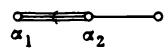
\includegraphics[keepaspectratio]{images/part002_d2921928.jpg}}

\begin{enumerate}
\def\labelenumi{(\Alph{enumi})}
\setcounter{enumi}{21}
\tightlist
\item
  \(R^{\prime}\) is the set of vectors
\end{enumerate}

\[
\pm \alpha_ {1}, \quad \pm (\alpha_ {1} + \alpha_ {2}), \quad \pm (2 \alpha_ {1} + \alpha_ {2}), \quad \pm \frac {1}{3} \alpha_ {2},
\]

\[
\pm \frac {1}{3} (3 \alpha_ {1} + \alpha_ {2}), \quad \pm \frac {1}{3} (3 \alpha_ {1} + 2 \alpha_ {2}).
\]

\[
  \Phi_ {\mathrm{R}} (x, y) = \frac {(x | y)}{24}, \quad \gamma (\mathrm{R}) = 48.
\]

\begin{enumerate}
\def\labelenumi{(\Roman{enumi})}
\setcounter{enumi}{5}
\tightlist
\item
  Fundamental weights:
\end{enumerate}

\[
\omega_ {1} = 2 \alpha_ {1} + \alpha_ {2}, \quad \omega_ {2} = 3 \alpha_ {1} + 2 \alpha_ {2} = \tilde {\alpha}.
\]

\begin{enumerate}
\def\labelenumi{(\Roman{enumi})}
\setcounter{enumi}{6}
\tightlist
\item
  Sum of the positive roots:
\end{enumerate}

\[
2 \rho = 2 (5 \alpha_ {1} + 3 \alpha_ {2}).
\]

\begin{enumerate}
\def\labelenumi{(\Roman{enumi})}
\setcounter{enumi}{7}
\item
  \(\mathrm{P}(\mathrm{R}) = \mathrm{Q}(\mathrm{R})\) . Connection index: 1.
\item
  Exponents: 1, 5.
\item
  W(R): the dihedral group of order 12.
\item
  and (XII): A(R) = W(R). \(w_{0} = -1\) .
\item
  Cartan matrix:
\end{enumerate}

\[
\left( \begin{array}{c c} 2 & - 1 \\ - 3 & 2 \end{array} \right)
\]

